\section{Optimization}
\begin{itemize}
    \item General information about optimization
    \item peephole optimization
    \begin{itemize}
        \item Optimize target code
        \item because we use circuit graph for simplicity
    \end{itemize}
    \item Some ``native'' optimizations
    \begin{itemize}
        \item Constant folding
        \item \dots
    \end{itemize}
\end{itemize}

\subsection{Optimization Rules}
\begin{itemize}
    \item Described in Sec.~\ref{sec:background_circuitOptimization}
\end{itemize}

\subsection{Circuit Graph}
\label{sec:concept_circuitGraph}
% Quick link to paper: https://quantum-journal.org/papers/q-2023-11-08-1176/pdf/
While it is possible to directly apply optimizations to the program code or internal representation of that code, this approach can be tedious and error prone. For example, the easiest approach would be to iterate over the code and search for code sequences with more efficient but equivalent alternatives, similar to the peephole optimization pattern on classical computers presented in Sec.~\ref{sec:background_codeOptimization}. However, two consecutive gates operating on a single wire may be separated by multiple gate applications on different wires in the programmatic description. Therefore, many simple optimization rules may not be applied when using a simplistic algorithm. A more complex approach would be too subdivide the program into lists of gate application where the wires being operated on by each list are disjunct. While this approach can result in the application of more optimization rules, it will also miss possible applications and already requires a complex implementation. Furthermore, improving on this method only increases its complexity and, in turn, makes it more prone to errors. Therefore, the language does not directly apply the optimizations to the program but uses a circuit graph description, based on the graph described by Kreppel et al.~\cite{KMO*23}, to apply the optimizations.

The circuit graph is a graphical description of a quantum graph; it is a acyclic and directed graph. For each qubit in the circuit, there exist both an input node and an output node. Furthermore, each input node as exactly one outgoing vertex while each output node as exactly one incoming vertex. Besides the input and output nodes, all other nodes represent gates in the circuit. All gate nodes the number of incoming vertices is equivalent to the number of outgoing vertices. Additionally, the number of incoming, or outgoing, vertices is the same as the number of parameters of the gate. Importantly, in this case, any qubits controlling the application of the gate, \eg the first qubit in a controlled-not gate, do also count to the number of parameters. In turn, their exists a vertices pair of an incoming and outgoing vertex each that represent a qubit to which the gate is applied. Therefore, for each qubit, there exists one path from its input node to its output node such that all gates that are applied to it are visited in order of application.

An example of a simple, unoptimized circuit graph is depicted in Fig.~\ref{fig:circuit_graph_unoptimized}. For simplicity, all applied gates are depicted in their corresponding node of the circuit graph. The circuit consist of three qubits, $q_0$, $q_1$, and $q_2$; their input and output nodes are depicted on the left and right of the graph respectively and are labeled with the corresponding qubit. Firstly, an $X$ is applied to the first qubit $q_0$. Than, a controlled-not gate is applied to the first two qubits $q_0$ and $q_1$, where $q_0$ is the controlling qubit. Simultaneously, two Hadamard gates $H$ are applied to the third qubit $q_2$. Lastly, another $X$ gate is applied to the first qubit $q_0$ while another controlled-not gate is applied to the second and third qubits $q_1$ and $q_2$. In this case, the second qubit $q_1$ is the controlling qubit.
\begin{figure}[htp]
    \centering     
    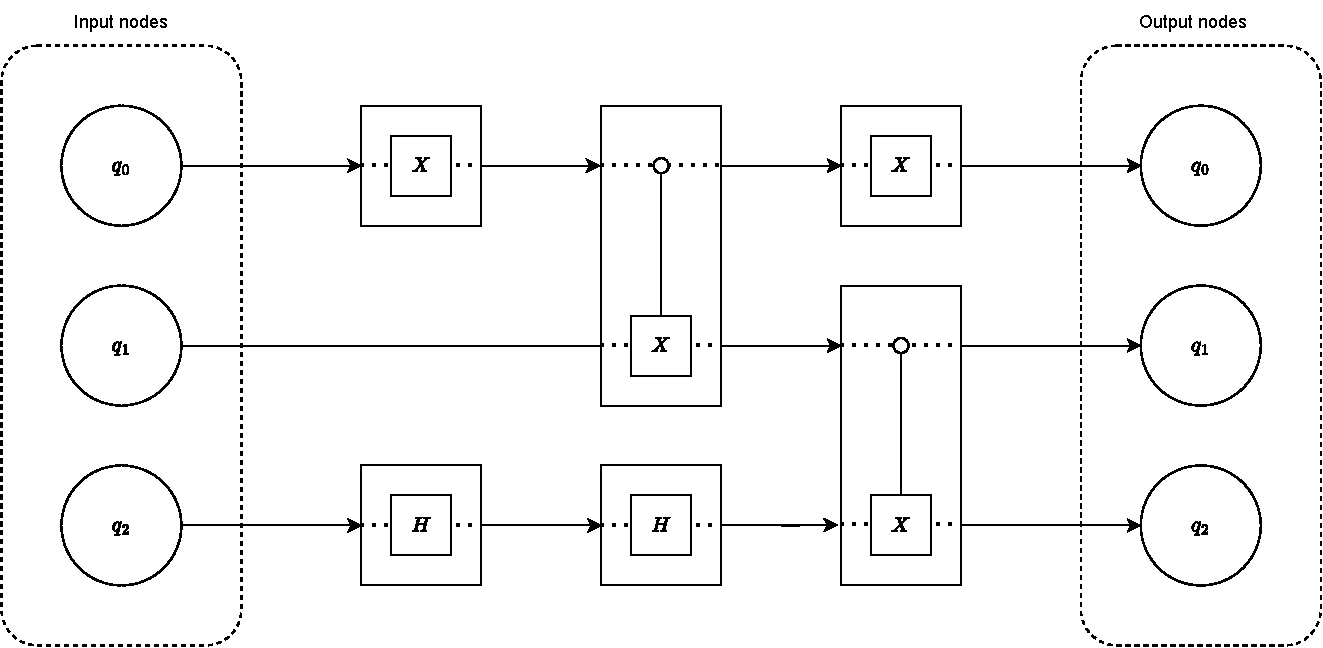
\includegraphics[width=.9\textwidth]{../figures/circuit_graph_unoptimized.pdf}
    \caption{An example of a simple, unoptimized circuit graph.}
    \label{fig:circuit_graph_unoptimized}
\end{figure}

When using the circuit graph to optimize the quantum program, the first step is to systematically construct the graph from the program. The creation of the graph starts with the input and output nodes for each qubit in the circuit. For each declaration of a qubit in the program, a input and output node pair is created. If a register is declared, a pair is created separately for each qubit in the register, \ie for a register with size $n$, $n$ pairs are created in total. Next, the gate applications in the program can be iterated. For each gate application, a corresponding gate node is created. To insert this node into the graph, each qubit parameter requires an incoming vertex to this node and a corresponding outgoing vertex from the node. Additionally, the incoming node must come from the gate that was previously applied to the qubit or the input node if no gate was applied yet. Similarly, the outgoing gate must lead to the either the next applied gate or the corresponding output. Therefore, for each qubit, the vertex coming into the output node can be diverted to the gate node and an outgoing vertex from the gate to the output node can be created. Repeating this step for all gate applications in the program result in the circuit graph.  

The next step in the optimization process is the application of optimization rules, in this case peephole optimizations, to the circuit graph. To accomplish this, subgraphs of the graph need to be iterated systematically. Then, each subgraph is checked for an equivalent but more efficient or cost-effective alternative. If an alternative is found, the subgraph is replaced with it. In our case, we iterate over all possible subpaths of all qubit paths up to a certain length; this length depends on the maximum number of nodes that are affected by an optimization rule. A qubit path is a path that starts at the input node of a qubit and ends in the corresponding output node. Furthermore, it visits only the nodes corresponding to the gates that are applied to the qubit in the correct order. However, optimizing parts of the circuit may enable further optimizations. For example, after removing a gate combination, two previously separated Hadamard gates may now represent a null gate combination which can, in turn, also be removed. Therefore, the process needs to be repeated until no more optimizations were applied.

Example ...

Lastly, construct program from optimized circuit graph \dots 